% Asset ID: AS1AlgebraicMethodsProofTikZ-004
% Source: Chapter 7b screenshots PDF pages 1 to 3 + transcript overview
% Related lesson section: Big Picture Explanation; Syllabus Gap Check
% Purpose: Four proof-type cards with proof by contradiction labelled as A2/future context.

\documentclass[tikz,border=8pt]{standalone}
\usepackage{amsmath}
\usetikzlibrary{positioning}
\begin{document}
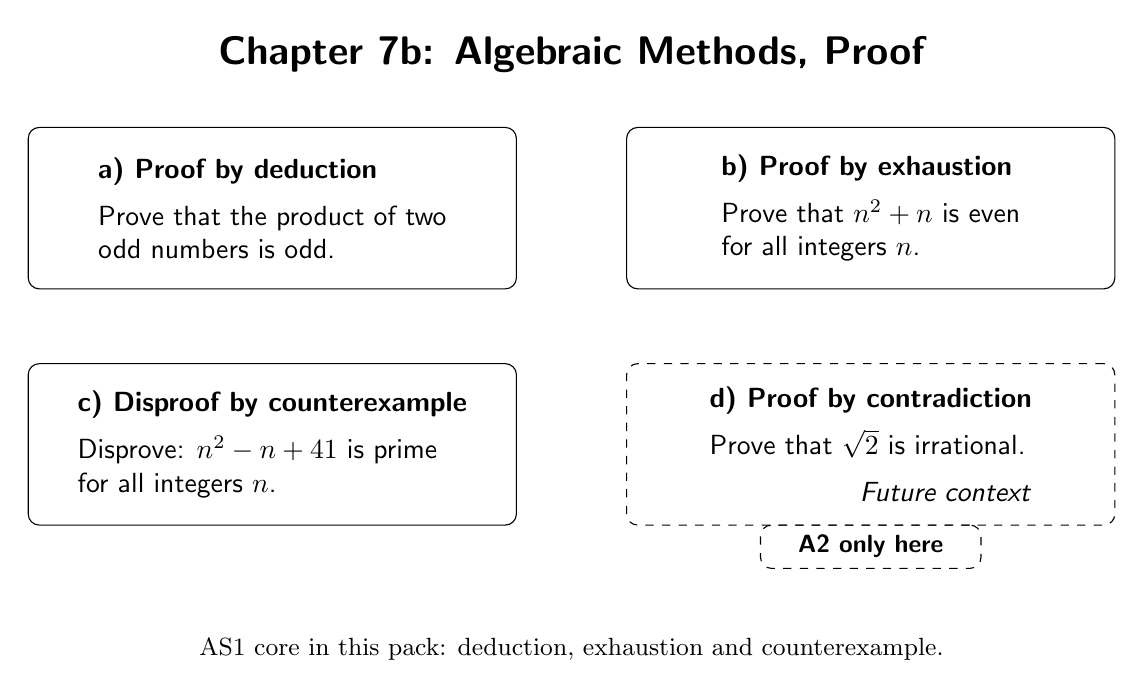
\begin{tikzpicture}[font=\sffamily,card/.style={draw,rounded corners,align=left,minimum width=6.2cm,minimum height=2.05cm,inner sep=8pt},future/.style={draw,dashed,rounded corners,align=left,minimum width=6.2cm,minimum height=2.05cm,inner sep=8pt},tag/.style={draw,dashed,rounded corners,align=center,minimum width=2.8cm,minimum height=0.55cm,inner sep=3pt,font=\sffamily\bfseries\small}]
\node[font=\sffamily\bfseries\Large, align=left] at (0,4.2){Chapter 7b: Algebraic Methods, Proof};
\node[card] at (-3.8,2.25){\textbf{a) Proof by deduction}\\[5pt]Prove that the product of two\\odd numbers is odd.};
\node[card] at (3.8,2.25){\textbf{b) Proof by exhaustion}\\[5pt]Prove that \(n^2+n\) is even\\for all integers \(n\).};
\node[card] at (-3.8,-0.75){\textbf{c) Disproof by counterexample}\\[5pt]Disprove: \(n^2-n+41\) is prime\\for all integers \(n\).};
\node[future] at (3.8,-0.75){\textbf{d) Proof by contradiction}\\[5pt]Prove that \(\sqrt{2}\) is irrational.\\[5pt]\hfill \textit{Future context}};
\node[tag] at (3.8,-2.05) {A2 only here};
\node[align=center, font=\small] at (0,-3.35){AS1 core in this pack: deduction, exhaustion and counterexample.};
\end{tikzpicture}
\end{document}
